\documentclass[11pt, english]{article}              
        \usepackage{geometry}
                \geometry{                          
                        a4paper,total={210mm,297mm},
                        tmargin=40.8mm,
                        bmargin=40.8mm,
                        lmargin=32.6mm,
                        rmargin=32.6mm,
                }

        \usepackage{titlesec}         
                \titleformat{\section}
                        {\normalfont\fontsize{18}{16}\bfseries}{\thesection}{0.5em}{}
                \titleformat{\subsection}
                        {\normalfont\fontsize{14}{16}\bfseries}{\thesubsection}{1em}{}
                \titleformat{\subsubsection}
                        {\normalfont\fontsize{11}{16}\bfseries}{\thesubsubsection}{1em}{}

        \usepackage{longtable}
        \usepackage{multirow}

        \usepackage[labelfont=bf,textfont=bf,font=small,skip=8pt]{caption}

        \setlength{\parindent}{0pt}
        \renewcommand{\baselinestretch}{1.25}
       	\usepackage{setspace}

        \usepackage{amsmath}
        \usepackage{amssymb}

        \usepackage{graphicx}

\begin{document}

\pagenumbering{gobble}

        \title{\textsc{AG432 Financial Quantitative Methods\\ Coursework Assignment}}
        \author{\textsc{Lewis Britton}}
        \date{\textsc{Academic Year 2020/2021}}
        \maketitle

\newpage

\pagenumbering{roman}

        \renewcommand{\contentsname}{Table of Contents}

        \tableofcontents

\newpage

\pagenumbering{arabic}

\section{J.P. Morgan \& The Volcker Rule}

	\subsection{Background to The Volcker Rule}

	In 2010, during the controversial Obama Administration, the Dodd-Frank Wall Street Reform and Consumer Protection Act was passed by Congress in response to the 2008 financial crisis. Generally, the Dodd-Frank Act was targeted at banks, mortgage lenders, and credit rating agencies – for example, by creating the Securities and Exchange Commission Office of Credit Ratings to regulate ratings. Section 619 of this act finds the topic of discussion, the Volcker Rule (Congressional Research Service, 2017). The Volcker Rule focuses solely on banks in this context. It was brought into effect in early 2014, stating that banks must provide full compliance by July 2015.

	\subsection{Purpose of The Volcker Rule}

	As with the Dodd-Frank Act, the Volcker rule's primary aim was to prevent any close repeat of the 2008 financial crisis. In effect, the rule was created to protect and serve the clients and consumers associated with banks. More specifically, it is designed to regulate banks to the degree of blocking proprietary trading with and ownership in hedge funds and private equity funds that are ``too risky'' (Congressional Research Service, 2017). This describes the scenarios where banks may have been using their own accounts to invest purely for capital gain instead of standard commission-based client trades. Therefore, this implies that the prohibited operations that were once practised did not benefit the bank's clients. The rule also extended to certain derivatives that were contributory to the 2008 crisis, such as Credit Default Swaps (CDS). These were all factors that tended to blur the line between commercial and investment operations within banks during the 2008 crisis (Thakor, 2012). The Volcker Rule aimed to clarify this line and make the distinction visible again, which was once the case until the Glass-Steagall Act's removal in 1999.

	\subsection{J.P. Morgan's Pre-2008 Operations}

	Concerning the J.P. Morgan article, the investment bank is portrayed as having a personal bias in relation to the Las Vegas car dealer, Greg Burk. It is suggested that JP Morgan was border-line dishonest with this gentleman simply for access to his funds. This relates to the Volcker Rule's primary idea, where banks are attempting to use clients' cash for undercalculated self-gain; further, using clients' cash for large internal investment opportunities. It was alleged that this was far from the first case of this behaviour within JP Morgan.\\

	It was suggested that JP Morgan were creating portfolios of perhaps naïve clients who are willing to invest millions of dollars without being fully on-board with the use of their funds in a risky manner between JP Morgan and hedge funds. This violated good practice and would therefore require regulation such as the Volcker Rule to overcome. JP Morgan's stake in Highbridge, a large investment group, was growing. Not only with regards to JP Morgan's ownership share in them but, with a huge portion of their assets being provided by the aforementioned operations of JP Morgan. This almost tripled the asset value of Highbridge. This is clearly the kind of thing the Volcker Rule was aiming to protect against. JP Morgan was using the financial ease of internal operations, Highbridge and clients' cash to greatly benefit themselves but leaving very little of the reward to their clients, such as Mr Burk. Directly linking to the Volcker Rule: JP Morgan's investment decisions were not made in favour of the clients; they had their own best interests in mind.\\

	This led to the idea of distrust surrounding JP Morgan. They continued to make growing profits in each new investment, and subsequently, it could be argued that the fees they were charging clients were heavily weighted to the profits they were making for themselves, as opposed to the payoffs for their clients. In practice: they arguably were manipulating relationships with clients. This was seen where Mr Burk's portfolio was experiencing fairly average performance; however, fees were huge, and the bank was moving tens of millions of Mr Burk's cash through its own Highbridge etc. This continued to benefit JP Morgan primarily and was reflected in Mr Burk's rising fees, leading to his confusion. This was again, heavily based around lack of disclosure and required regulation such as the Volcker Rule for urgent amendment, from the clients' point of view. All of these factors point directly to divisions of the Volcker Rule: regulating the requirement for making investment decisions in favour of the client; for not engaging in investment opportunities/trades where they have a significant advantage and; providing full disclosure of methods and performance to their clients.

	\subsection{J.P. Morgan's Post-2008 Operations}

	After the 2008 crisis, Highbridge's volume of private bank clients significantly decreased as other outside investors began to return. At this point, the majority of JP Morgan's private bank clients held funds in places which are not associated with Highbridge. Newly reduced fees were suggested to be utilised to encourage increased volume in other areas in order to build back a large asset basis. JP Morgan's alternative strategies with more transparency in regard to trading with their clients' best interests in mind were implemented to attempt to find a new method of optimising investments. It is now clear that JP Morgan continue to attempt to find methods to avoid the Volcker Rule. Clearly, JP Morgan's historic tactics have been made transparent by the introduction of the Volcker Rule, reinforced by JP Morgan's settlement with the Securities and Exchange Commission for \$150m regarding their pre-Volcker-Rule operations.

	\subsection{Effect \& Criticisms}

	In short, the Volcker Rule has been fairly successful but highly criticised. The primary criticism is that the Volcker Rule is too vague regarding who and where operations can be conducted. Alternatively, more specifically, prohibited. Corporations who still engage in the aforementioned propriety trading methods are majorly less regulated and smaller with less power (Whitehead, 2011). However, these entities have also been found to have a large connection to bigger banks; usually, ones which rely on hedge/private equity funds etc. (Whitehead, 2011). This means that although the Volcker Rule has been effective to a reasonable degree on a larger scale, in the context of JP Morgan, for example, its regulation still leaving large loopholes through which banks can more indirectly engage in their former activities.

\newpage

\section{Hedge Fund Performance}

	\subsection{Introduction to Hedge Fund Performance}

	It has been argued that when observing the performance and returns of hedge funds, there are a number of internal firm and external economic factors which play a role. These include characteristics such as; fund size, the age of the fund, its disclosure requirements, their lockup period etc. (Frumkin, Venegrift, 2009). Furthermore, there has been evidence regarding hedge fund style and strategy, such as the targeting of the right type of investors (O'Doherty et al., 2017). Analysis of both of these primary factors aims to provide investors with the information they need to make the right investments for themselves based on how the fund managers operate. That is, do their philosophies match?

	\subsection{Hedge Fund Characteristics}

	In the context of both successful and unsuccessful states of an economy, Stafylas and Andrikopoulos (2019) put forward various hypotheses regarding the characteristics of hedge funds. These include: [1] smaller funds which have been established for less time will, on average, outperform larger firms which have been established for longer, in all states of the economy; [2] hedge funds yield positive and similar returns regardless of their characteristics and the economic state; and [3], throughout weak economic states, hedge funds decrease market exposure regardless of their characteristics. In order to support or debate these points, we explore the following.\\

	Regarding the first hypothesis stated, Meredith (2007) found evidence that across a large sample of hedge funds, the majority of smaller – lower market capitalisation, younger funds outperformed larger and older ones primarily due to the classic assumption that these firms are riskier due to their lack of credibility and investor trust in their early days. However, Schneeweis et al. (2002) found that when observing larger firms who had built a better reputation – primarily located in the large trading sectors – found greater returns and outperformed. This observation could have included some bias towards the more reputable larger firms as opposed to just all large, old firms. However, it still makes the point that utilising higher trading volumes and sizeable investor wealth will have a significantly positive effect on hedge fund performance.\\

	Furthermore, regarding disclosure requirements, Ling (1999) mentions those who utilise redemption restrictions in order to control investors' cash withdrawal increasingly outperform funds which do not practice this. In evidence, firms who practice this method tend to be more established and have built a better relationship with their investors and clients. Hence, in effect, they end up holding their investors for more prolonged periods; sealing in their more of their cash over time, so the disclosure of this practice tends to show investors that these firms are trustworthy over the long term implying that they have created a foundation for themselves in the same respect.\\

	Additionally, Di Tommaso and Piluso (2018) find that, in a good economic state, hedge funds which hold a large volume of illiquid assets outperform ones which hold a majority of liquid ones. Arguably, this is primarily due to the liquidity premium, which is attached to these assets, meaning that there will be a premium charged to compensate for the risk of holding an illiquid asset. Of course, this outperformance method is quite volatile, and although a premium is gained, many of these investments may remain illiquid for an extended period and therefore be harder to sell. Siegmann and Stefanova (2017) find that in a poor economic state; however, this does not hold as the funds which hold illiquid assets tend to offer liquidity discounts.

	\subsection{Hedge Fund Style \& Strategy}

	In evidence, there has been a positive relationship found between the performance of funds and the management fees (Joenv\"{a}\"{a}r\"{a} et al., 2012). This could be attributed to many factors; however, one of the most discussed is the overall skill of the manager. Most often, managers with a higher skill level will charge higher fees and will drive higher returns. The question here is, does this stagnate? However, this is again contradicted by the findings of Schneeweis et al. (2002), who said that there was no apparent relationship between management fees and performance. This also could contain some bias in more reputable funds explored by Schneeweis in the sense that the lack of variation in management fees in the sample used does not allow enough room for accountability. Whereas, studying more intermediate funds, for example, could show more variation in management fees while funds are still exponentially growing and are riskier, could highlight the aforementioned positive relationship between fees and performance, due to the initial incentive driver.\\

	Furthermore, funds which use fees, minimum investments, etc., also tend to outperform funds which do not (Stafylas, Andrikopoulos, 2019). This is again primarily attributed to the individual relationship with the investor and their investment philosophy. It is regarded as a strategy put in place by the fund manager to select the correct investors for their fund. As is the case with most firms in any industry seeking investment, they wish to find more trustworthy and consistent investors. In practice, it is found that firms who practice this strategy tend to hold onto wealthier investors who want to settle their cash in one location for longer periods and therefore, the more the hedge fund makes itself look, almost, 'premium', the more of these investors they will attract.\\

	In short, smaller funds who are more open to taking risks to build their folios may outperform the larger ones but, in more volatile patterns and for less consistent time periods. The characteristic-based factors of a hedge fund speak for themselves and are mainly what drives their reputation and long-term performance. Hedge fund strategy is important for making the correct decision at a given period of time and ultimately, is what will create their reputation in the first place and maintaining it. A primary takeaway from this is that reputable firms are successful. The trust investors have in the fund manager, and the perceived 'class' of the hedge fund play a huge part in drawing in wealthy investors and driving higher fund performance. In a way, this context contradicts expectations to be otherwise known. The more expensive the fee, the higher the minimum investment in effect leads to more attraction, trust and long-term high performance.

\newpage

\section{Hedge Fund Performance Analysis}

	Aim: investigate effect of various (9) factors (11 variables) on whether a hedge fund is live/defunct. Based on a sample of 1000 live and 1000 defunct funds (2000 observations), using logistic regression (Appendix 1).

	\begin{center}
		\scriptsize
	\begin{longtable}{p{2cm}p{3cm}p{3cm}p{5cm}}
		\textbf{Purpose} & \textbf{Name} & \textbf{Type} & \textbf{Description}	\\
		\hline
		Dependent & Live/Defunct & Categorical Binary & \tiny Shows whether a hedge fund is active or no longer in operation. 0 represents a live hedge fund and 1 defunct one. As 1 is defunct, we are attempting to explain defunct.\\
		Explanatory & Management Fee & Continuous Numerical & \tiny Represents percentage (\%) paid to hedge fund managers. The percentage is dependent on the Assets Under Management (AUM) and is measured relative to it. This is the sum of all the market values of the investments managed by the hedge fund.\\
		Explanatory & Incentive Fee & Continuous Numerical & \tiny Represents the fee which is charged by a hedge fund manager based on the performance of the fund. This is heavily based on comparison to a benchmark such; higher incentive fees are positively correlated with outperformance of market indices, for example. It can also be based heavily around Net Asset Value. This again is a percentage represented in decimal form.\\
		Explanatory & High-Water Mark & Categorical Binary & \tiny Shows whether a fund has a High-Water Mark in a given year. A value of 1 shows it does, 0 shows it does not.\\
		Explanatory & Leverage & Categorical Binary & \tiny Shows whether a hedge fund uses leveraged financing or not. 1 represents yes, 0 represents no.\\
		Explanatory & Personal Capital & Categorical Binary & \tiny Shows whether a hedge firm uses personal capital from its manager. 1 represents yes, 0 represents no.\\
		Explanatory & Currency Exposure & Categorical Binary & \tiny Shows whether a hedge fund is exposed to foreign currency or not. 1 shows it is, 0 shows it is not.\\
		Explanatory & Lock-Up Period & Continuous Numerical & \tiny Represents the period where investors aren't allowed to sell or redeem shares held in investment s with the hedge fund. A longer Lock-Up Period gives managers more time to exit investment or omit ones which show to skew their portfolios too quickly. This is measured in days.\\
		Explanatory & Redemption Period & Continuous Numerical & \tiny Represents the period under which, before the maturity date, an investor must notify their fund manager that they wish to redeem repayment of a security. This is measured in days.\\
		Explanatory & Legal Structure & Non-Numerical & \tiny Non-numerical descriptor based on the type of firm a hedge fund is legally registered as. This requires three dummy variables as follows. Their derivation can also be seen below this table.\\
		Explanatory & D\_Limited* & Categorical Binary & \tiny 1 = `Limited Company'; 0 = = Not\\
		Explanatory & D\_UnitTrust* & Categorical Binary & \tiny 1 = `Unit Trust'; 0 = Not\\
		Explanatory & D\_UnitTrustB* & Categorical Binary & \tiny 1 = `Unit Trust B-Scheme'; 0 = Not\\
		\hline
		\caption{Sample \& Variables}
	\end{longtable}
	\end{center}

	Furthermore:

	\begin{itemize}
		\scriptsize
	\setlength\itemsep{0cm}
		\item \{`Limited Company'; `Unit Trust'; `Unit Trust B-Scheme'; `Other'\} $\in$ `Legal Structure';
		\item N\_Categories = 4;
		\item We need (N\_Categories $-$ 1) dummies so;
		\item Dummy Variables = 3;
		\item Reference = `Other' (does not require dummy as triple-0 implies ``Other is active'');
		\item Example shown below (Figure 2).
	\end{itemize}

	\begin{table}[h]
		\scriptsize
		\renewcommand{\arraystretch}{1.25}
	\begin{center}
	\begin{tabular}{p{3cm}p{3cm}p{3cm}p{3cm}}
		& \textbf{D\_Limited} & \textbf{D\_UnitTrust} & \textbf{D\_UnitTrustB}\\
		\hline
		`Limited Company' & 1 & 0 & 0\\
		`Unit Trust' & 0 & 1 & 0\\ 
		`Unit Trust B-Scheme' & 0 & 0 & 1\\
		`Other' & 0 & 0 & 0\\
		\hline
	\end{tabular}
		\caption{Example Dummy Variables for `Legal Structure'}
	\end{center}
	\end{table}

	\newpage

	\subsection{Regression Results}

	\begin{table}[h]
		\scriptsize
		\renewcommand{\arraystretch}{1.25}
	\begin{center}
	\begin{tabular}{p{3cm}p{1.75cm}p{1.75cm}p{2cm}c}
		& \textbf{coefficient} & \textbf{std.err} & \textbf{t-ratio} & \textbf{significance state}\\
		\hline
		const & 0.2898 & 0.0691 & 4.1976 & Yes\\
		Management Fee & 7.7129 & 3.8728 & 1.9915 & Yes\\
		Incentive Fee & 6.5595 & 0.4452 & 14.7354 & Yes\\
		High-Water Mark & -3.5382 & 0.1329 & -26.6260 & Yes\\
		Leverage & 0.0559 & 0.0884 & 0.6322 & No\\
		Personal Capital & 1.6609 & 0.1161 & 14.3007 & Yes\\
		Currency Exposure & -4.2620 & 1.0419 & -4.0907 & Yes\\
		Lock-Up Period & -0.0471 & 0.0195 & -2.4074 & Yes\\
		Redemption Period & -0.0278 & 0.0022 & -12.6752 & Yes\\
		D\_Limited & -0.2212 & 0.4845 & -0.4567 & No\\
		D\_UnitTrust & -1.4494 & 0.4422 & -3.2776 & Yes\\
		D\_UnitTrustB & -1.8548 & 1.1071 & -1.6753 & No\\
		\hline
	\end{tabular}
		\caption{t-test Results}
	\end{center}
	\end{table}

	This regression analysis observes the following hypotheses:\\

	\textbf{H}$\mathbf{_0}$: Observed factor does not have an effect on probability of a fund being defunct\\
	\textbf{H}$\mathbf{_A}$: Observed factor does have an effect on probability of a fund being defunct\\

	We know that if the magnitude of the produced t-value is greater than 1.96 ($|t-ratio|>1.96$), we can reject the null hypothesis in favour of the alternative hypothesis saying that there is statistical significance. As we are using a critical value of 1.96 (Appendix 2), this is therefore relative to the 95\% confidence interval. Referring to the above figure (Figure 3), we make the following observations. Results estimated using MATLAB (Appendix 3).

		\subsubsection{Constant}

	We observe a constant of 0.2898 meaning that if there were no measure of explanation for whether a fund is live/defunct, the odds of it being defunct would be 0.2898.

		\subsubsection{t-ratios}

	Management Fee, Incentive Fee, Lock-Up Period and Redemption Period are the continuous numerical variables which are significant. We see that their t-values are 1.9915, 14.7354, -2.4074 and -12.6752 respectively. Therefore the null hypotheses that management fees and incentive fees have no effect on whether a fund is defunct can be rejected in favour of the alternative hypotheses stating that they do.\\

	High-Water Mark, Personal Capital, Currency Exposure and D\_UnitTrust are the dummy variables which all present t-values with magnitude greater than 1.96; -26.6260, 14.3007, -4.0907 and -3.2776 respectively. Therefore the null hypotheses that they have no statistical significance in explaining whether a fund is defunct can also be rejected in favour of the alternative hypotheses stating that they do.\\

	Finally, we observe t-values with magnitude less than 1.96 from the variables Leverage, D\_Limited and D\_UnitTrustB. Therefore we fail to reject the null hypotheses that if a fund is a Limited Company and if a fund is a Unit Trust B-Scheme have no statistical significance in explaining whether a fund is defunct.

		\subsubsection{Coefficients}

	\textbf{Management Fee$\mathbf{^N}$\footnote{Note that $\mathrm{^N}$ denotes Numerical Continuous Variables}}: 7.7129

	\begin{itemize}
	\setlength\itemsep{0cm}
		\item[i] Positive correlation (relationship) with Live/Defunct
		\item[ii] For a 1 unit increase of management fee, the odds of a fund being defunct \textit{increases} by 7.7129 units
		\item[iii] ``The higher the management fee, the \textit{more} probable it is that a fund is defunct'' 
		\item[iv] Intuitively, the more funds which are used to pay management fees, the less capital available for reinvestment and housing new clients. Investors may also be offput by this, knowing that they may find higher returns with lower management fee funds.
	\end{itemize}

	\textbf{Incentive Fee$\mathbf{^N}$}: 6.5595

	\begin{itemize}
        \setlength\itemsep{0cm}
		\item[i] Positive correlation (relationship) with Live/Defunct
		\item[ii] For a 1 unit increase of incentive fee, the odds of a fund being defunct \textit{increases} by 6.5595 units
		\item[iii] ``The higher the incentive fee, the \textit{more} probable it is that a fund is defunct''
		\item[iv] Intuitively, in a similar way to management fees, increasing incentive fees reduces capital available for investment and cash retention. Further, making the financial position more volatile.
	\end{itemize}

	\textbf{Lock-Up Period$\mathbf{^N}$}: -0.0471

        \begin{itemize}
        \setlength\itemsep{0cm}
                \item[i] Negative correlation (relationship) with Live/Defunct
		\item[ii] For a 1 unit increase of lock-up period, the odds of a fund being defunct \textit{decreases} by 0.0471 units
		\item[iii] ``The longer the lock-up period, the \textit{less} probable it is that a fund is defunct''
                \item[iv] Longer Lock-Up Periods allow funds to retain investor capital for longer, giving them more freedom in the case of financial distress.
        \end{itemize}

	\textbf{Redemption Period$\mathbf{^N}$}: -0.0278

        \begin{itemize}
        \setlength\itemsep{0cm}
                \item[i] Negative correlation (relationship) with Live/Defunct
		\item[ii] For a 1 unit increase of redemption period, the odds of a fund being defunct \textit{decreases} by 0.0278 units
		\item[iii] ``The longer the redemption period, the \textit{less} probable it is that a fund is defunct''
                \item[iv] Longer Redemption Period allows funds to put more effort into effective liquidation of investors assets, providing more loyalty and trust in the long-run. Also, safer procedures in the case of financial distress.
        \end{itemize}

	\textbf{High-Water Mark$\mathbf{^D}$\footnote{Note that $\mathrm{^D}$ denotes Dummy Variables}}: -3.5382

        \begin{itemize}
        \setlength\itemsep{0cm}
                \item[i] Negative correlation (relationship) with Live/Defunct
		\item[ii] Funds with a high-water mark are 3.5382 units \textit{less} probable of being defunct
		\item[iii] ``If a fund has a high-water mark it is \textit{less} likely to be defunct''
                \item[iv] Having a HWM can increase the funds available to a firm in financial distress as it restricts the management fees unless they outperform previous NAV. This also provides an incentive to outperform from a management fee perspective.
        \end{itemize}

	\textbf{Personal Capital$\mathbf{^D}$}: 1.6609

        \begin{itemize}
        \setlength\itemsep{0cm}
                \item[i] Positive correlation (relationship) with Live/Defunct
		\item[ii] Funds which use personal capital are 1.6609 units \textit{more} probable of being defunct
		\item[iii] ``If a fund uses personal capital it is \textit{more} likely to be defunct''
                \item[iv] If a fund relies heavily on its management's personal cash, it may be more prone to defunct as it is exposed not only to corporate risk but also to personal financial risk related to the managers. If a fund is majorly personally financed and the managers find themselves in financial trouble/bankruptcy, so too may the fund. They might not have any cash left to [1] bail themselves out of trouble or [2] bail the fund out.
        \end{itemize}

	\textbf{Currency Exposure$\mathbf{^D}$}: -4.2620

        \begin{itemize}
        \setlength\itemsep{0cm}
                \item[i] Negative correlation (relationship) with Live/Defunct
		\item[ii] Funds with currency exposure are 4.2620 units \textit{less} probable of being defunct
                \item[iii] ``If a fund is exposed to foreign currency, it is \textit{less} likely to be defunct''
                \item[iv] Having exposure to foreign currency could amplify the effect in either way in the case of financial distress. Using foreign currency could allow funds to restructure and save themselves from default however, it could also expose them to greater risk all over the board. In this sample though, it's the former.
        \end{itemize}

	\textbf{D\_UnitTrust$\mathbf{^D}$}: -1.4494

        \begin{itemize}
        \setlength\itemsep{0cm}
                \item[i] Negative correlation (relationship) with Live/Defunct
		\item[ii] Funds which are Unit Trusts are 1.4494 units \textit{less} in probable of being defunct
		\item[iii] ``If a fund is a Unit Trust, it is \textit{less} likely to be defunct''
                \item[iv] Unit Trusts use a more stable financial structure and a direct distribution of profits to unit owners so, they are more reliable in the long-run and also desirable to investors.
        \end{itemize}

	\subsection{Additional Factors}

	Although we have analysed various factors which have been proven to show a statistically significant effect on probability of live/defunct fund status, there are other externally discussed factors which can also have an effect on a fund's performance and their subsequent state of operation. First is the idea that funds which use a higher minimum investment may see a higher chance of defunct (Stafylas, Andrikopoulos, 2019). This is due to the fact that larger volumes of investors may be off-put buy the minimum investment and even may not have the liquidity to fund their investment with those particular funds. However, if funds employ tactics to focus their attraction to the correct investors, i.e. wealthier/larger-investment-oriented ones, that the sum of investment could outweigh the lack of attraction to the higher volumes. Minimum investment requirements can vary by many hundreds-of-thousands of dollars and therefore leave a large margin for investment decision to be swayed by this factor.\\

	Also is a factor very similar to the legal structure of a fund, whether or not it is SEC Registered. We know that registration in this regard would imply closer and more rigorous regulation and restrictions. A fund's registration with the SEC reflects a size greater than \$100m, highlighting a historically string fund performance and possible long life. This, in a way, contradicts the idea from earlier that smaller firms outperform larger ones due to their higher initial risk taking and larger payoffs (Meredith, 2007). As expected, this latter argument would not be likely to hold into long-term fund survival. We'd therefore expect larger more stable fund size to be positively related to fund livelihood.\\

	Furthermore, we can recall that Schneeweis et al. (2002) found that funds which had been established for longer (have a higher age) may present a positive relationship with their likelihood of being active or defunct now. Generally, if a fund has been around longer it has shown more stability and profitability over time and therefore has established a better long-term relationship with investors. This means they will also have gained the ability to use higher fees and higher minimum investments, possibly further contributing to their profitability and long-term financial stability and likelihood of survival.\\

	Finally, a factor called the `Main Strategy' has been found to contribute to liveliness/ defunct as it can contribute directly to risk (Lin, 2016). For example, if a fund employs a higher risk investment strategy as their primary focus, their overall risk can be biased and make them more probable of defunct.

\newpage

\section*{Appendices}

	\subsection*{Appendix 1: Logistic Regression Model}

	Logistic regression is used in this case as the dependent variable is binary and therefore violates rules and assumptions of OLS regressions. Logistic regression allows for a binary dependant variable by dropping further assumptions such as linearity and homoscedastic (constant) error terms. Fundamentally, the dependant variable is an 'event' and we wish to discover what effects the probability of it.

	$$\ln\left(\frac{p}{(1-p)}\right)\equiv\mathrm{logit}P=\alpha+\beta X+\varepsilon$$

	Where:\\
	$p$ = Probability of Event Occuring\\
	$\frac{p}{(1-p)}$ = Odds Ratio\\
	$\ln\left(\frac{p}{(1-p)}\right)$ = Log Odds Ratio (LOGIT)\\

	Probability of explanatories causing event:\\
	$p(y=1|x)=\frac{1}{1+E(-\alpha-\beta X)}$\\

	If/As:\\
	$\alpha+\beta X=0$: $p=0.5$\\
	$\alpha+\beta X$ Gets Bigger: $p$ Approaches 1\\
	$\alpha+\beta X$ Gets Smaller: $p$ Approaches 0

	\newpage

	\subsection*{Appendix 2: t-distribution Critical Values}

	\begin{center}
		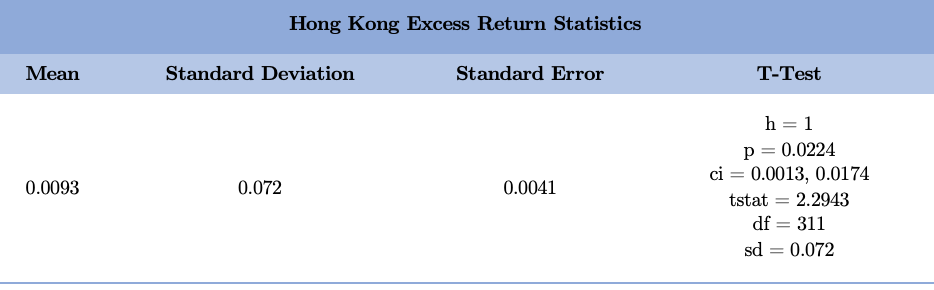
\includegraphics[height=12cm,width=13cm]{AG432-IMG/a.PNG}
	\end{center}

	\newpage

	\subsection*{Appendix 3: MATLAB Code}

	\% Reading the data and saving:\\
	\texttt{data = xlsxread(`\~{}/Documents/Fourth Year/Quantitative Methods/Assignment/ Project Data.xlsx')}\\

	\% Capturing all dependent variable Y:\\
	\texttt{Y = data(:,1);}\\

	\% Capturing all X explanatory variables in one matrix:\\
	\texttt{X = data(:,2:12);}\\

	\% Adding a column of ones (the constant) preceding the explanatories:\\
	\texttt{X = [ones(2000,1) X];}\\
	or\\
	\texttt{X = [ones(size(data,1)) X];}\\

	\% Estimate coefficients and standard error:\\
	\texttt{[coeff, stderr] = Logit(Y,X);}\\

	\% t-test estimations:\\
	\texttt{tvalues = coeff./stderr}

\newpage

\renewcommand\refname{Bibliography}

\begin{thebibliography}{9}

	\bibitem{a}
		Congressional Research Service. (2017).
		\textsl{The Dodd-Frank Wall Street Reform and Consumer Protection Act: Background and Summary.}
		Available At:
		https://fas.org/sgp/crs/misc/R41350.pdf
		(Accessed: 15/10/2020).

	\bibitem{c}
		Di Tommaso, C., Piluso, F. (2018).
		\textsl{The failure of hedge funds: an analysis of the impact of different risk classes.}
		Research in International Business and Finance. Volume 45. Issue 1. Pages 121-133.

	\bibitem{d}                    
                Frumkin, D., Vandegrift, D. (2009). 
                \textsl{The effect of size, age, beta and disclosure requirements on hedge fund performance.}
		Journal of Derivatives \& Hedge Funds. Volume 15. Pages 241-251.

	\bibitem{e}                    
                Joenv\"{a}\"{a}r\"{a}, R., Kosowski, R., Tolonen, T. (2012).
                \textsl{Revisiting ``stylized facts'' about hedge funds.}
		SSRN Working Paper.

	\bibitem{f}                    
                Lin, T. (2016). 
                \textsl{Before and After the Financial Crisis: Reevaluating Hedge Fund Survival Probability Model.}
		Joseph Wharton Scholars.

	\bibitem{g}                    
                Ling, B. (1999). 
                \textsl{On the performance of hedge funds.}
		Financial Analysts Journal. Volume 55. Pages 72-85.

	\bibitem{h}                    
                Meredith, J. (2007).
                \textsl{Examination of fund age and size and its impact on the hedge fund performance.}
		Derivatives Use. Trading and Regul. Volume 12. Issue 4. Pages 342-350.

	\bibitem{i}                    
                O'Doherty, M., Savin, N., Tiwari, A. (2017).
                \textsl{Hedge Fund Replication: A Model Combination Approach.}
		Review of Finance. Volume 21. Issue 4. Pages 1767-1804.

	\bibitem{j}                    
                Siegmann, A., Stefanova, D. (2017). 
                \textsl{The evolving beta-liquidity relationship of hedge funds.}
		Journal of Empirical Finance. Volume 44. Issue 1. Pages 286-303.

	\bibitem{k}                    
                Stafylas, D., Andrikopoulos, A. (2019).
                \textsl{Determinants of hedge fund performance during 'good' and 'bad' economic periods.}
		Research in International Business \& Finance. Volume 52.

	\bibitem{l}                    
		Schneeweis, T., Kazemi, K., Martin, G. (2002).                   
                \textsl{Understanding hedge fund performance: research issues revisited – part I.}
		The Journal of Alternative Investments. Volume 5. Issue 3. Pages 6-22.
			
	\bibitem{m}                    
                Thakor, A. (2012).
                \textsl{Incentives to Innovate and Financial Crises.}
		Journal of Financial Economics. Volume 103, Pages 130-143.

	\bibitem{n}                    
                t-table. (2020).
                \textsl{t-table – t-values.}
		Available At:
		http://www.ttable.org/.
		(Accessed: 01/11/20).

	\bibitem{o}                    
                Whitehead, C. (2011). 
                \textsl{The Volcker Rule and Evolving Financial Markets.}
		Harvard Business Law Review. Volume 39.

\end{thebibliography}

\end{document}
